\documentclass[11pt,twoside,a4paper]{article}
% http://www-h.eng.cam.ac.uk/help/tpl/textprocessing/latex_maths+pix/node6.html symboles de math
% http://fr.wikibooks.org/wiki/Programmation_LaTeX Programmation latex (wikibook)
%=========================== En-Tete =================================
%--- Insertion de paquetages (optionnel) ---
\usepackage[french]{babel}
\usepackage{a4}				 % pour la taille   
\usepackage[T1]{fontenc}	 % pour les font postscript
\usepackage{epsfig}		  % pour gerer les images
%\usepackage{psfig}
\usepackage{amsmath, amsthm} % tres bon mode mathematique
\usepackage{amsfonts,amssymb}% permet la definition des ensembles
\usepackage{float}		   % pour le placement des figure
\usepackage{verbatim}
\usepackage{longtable} % pour les tableaux de plusieurs pages
\usepackage[table]{xcolor} % couleur de fond des cellules de tableaux
\usepackage{lastpage}
\usepackage{multirow}
\usepackage{multicol} % pour {\'e}crire dans certaines zones en colonnes : \begin{multicols}{nb colonnes}...\end{multicols} 

% \usepackage[top=1.5cm, bottom=1.5cm, left=1.5cm, right=1.5cm]{geometry}
% gauche, haut, droite, bas, entete, ente2txt, pied, txt2pied
\usepackage{vmargin}
\setmarginsrb{1.0cm}{1.0cm}{1.0cm}{1.0cm}{15pt}{3pt}{60pt}{25pt}

\usepackage{lscape} % changement orientation page

%\usepackage{frbib} % enlever pour obtenir references en anglais
% --- style de page (pour les en-tete) ---
\pagestyle{empty}

\def\MainTitle{geNorNics}

% % % en-tete et pieds de page configurables : fancyhdr.sty

% http://www.trustonme.net/didactels/250.html

% http://ww3.ac-poitiers.fr/math/tex/pratique/entete/entete.htm
% http://www.ctan.org/tex-archive/macros/latex/contrib/fancyhdr/fancyhdr.pdf
\usepackage{fancyhdr}
\pagestyle{fancy}
% \newcommand{\chaptermark}[1]{\markboth{#1}{}}
% \newcommand{\sectionmark}[1]{\markright{\thesection\ #1}}
\fancyhf{}
\fancyhead[LE,RO]{\bfseries\thepage}
\fancyhead[LO]{\bfseries\rightmark}
\fancyhead[RE]{\bfseries\leftmark}
\fancyfoot[LE]{\thepage /\pageref{LastPage} \hfill
	\MainTitle 
\hfill 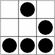
\includegraphics[width=0.5cm]{img/logo_glider.png} }
\fancyfoot[RO]{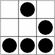
\includegraphics[width=0.5cm]{img/logo_glider.png} \hfill
	\MainTitle 
\hfill \thepage /\pageref{LastPage}}
\renewcommand{\headrulewidth}{0.25pt}
\renewcommand{\footrulewidth}{0.50pt}
\addtolength{\headheight}{0.5pt}
\fancypagestyle{plain}{
	\fancyhead{}
	\fancyfoot{}
	\renewcommand{\headrulewidth}{0pt}
}

%--- Definitions de nouvelles commandes ---
\newcommand{\N}{\mathbb{N}} % les entiers naturels

%--- Definitions de nouvelles couleurs ---
\definecolor{verylightgrey}{rgb}{0.8,0.8,0.8}
\definecolor{verylightgray}{gray}{0.80}
\definecolor{lightgrey}{rgb}{0.6,0.6,0.6}
\definecolor{lightgray}{gray}{0.6}

%============================= Corps =================================
\begin{document}

\setlength\parindent{0pt}

%% ~\\
\vfill

\begin{center}
	\textbf{ \MainTitle }~\\
	~\\~\\~\\
	\texttt{http://meliweb.net/creatures/}~\\
\end{center}

\tableofcontents

\vfill

~\\

\clearpage

\section*{Training Department\markboth{Training Department}{Training Department}}
\addcontentsline{toc}{section}{Training Department}

\subsection*{An Introduction to Norn Genetics\markboth{An Introduction to Norn Genetics}{An Introduction to Norn Genetics}}
\addcontentsline{toc}{subsection}{An Introduction to Norn Genetics}

\subsubsection*{Overview\markboth{Overview}{Overview}}
\addcontentsline{toc}{subsubsection}{Overview}

Ok, the first thing to remember is that genetics in Creatures$\texttrademark$ is /not/ like genetics in real life.

In people, animals, plants, etc. in our world, chromosomes are complex collections of base pairs defining tons of individual genes, each of which codes a specific protein used in the development and life processes of the organism.

In Creatures$\texttrademark$, there is a single 'chromosome' bearing around 320-350 'genes' that are basically sequences of computer instructions defined to mimic this development and these life processes.

That said, there's still an awful lot of interesting stuff to be learned about Norn genetics.

\subsubsection*{Gene Types and Subtypes\markboth{Gene Types and Subtypes}{Gene Types and Subtypes}}
\addcontentsline{toc}{subsubsection}{Gene Types and Subtypes}

In Creatures$\texttrademark$, there are three main groups, or types, of genes. Each of these groups has one or more subtypes of genes as well, for a total of thirteen separate sets of genes.
\begin{itemize}
	%% \setlength{\itemsep}{0pt} %% useful if babel is on english...
	%% \setlength{\parskip}{0cm} %% useful if babel is on english...
	\item Brain genes define the workings of the creatures' brains. There is a single subtype ('lobe'), but it is the most complex gene type.
	\item Biochemistry genes describe the way that the various chemicals are produced by and used within a creature during its lifetime. There are five subtypes of biochemistry genes.
	\item Creature genes define the way the creature looks, moves, and responds to its environment. There are seven subtypes.
\end{itemize} %% ~\\

\subsubsection*{Gene Files and Breeding\markboth{Gene Files and Breeding}{Gene Files and Breeding}}
\addcontentsline{toc}{subsubsection}{Gene Files and Breeding}

Unlike real-life animals, each creature (norn or grendel) has a genotype consisting of a single, haploid chromosome. When two creatures breed successfully, the following sequence occurs:
\begin{enumerate}
	\setlength{\itemsep}{0pt}
	\setlength{\parskip}{0cm}
	\item The two genome files (one from the mother, one from the father) are lined up for comparison.
	\item One or the other version of each gene is randomly selected from the two files.
	\item Errors such as mutations, duplications, or deletions may occur (depending on the gene -- some gene types do not allow any errors).
	\item The resulting genome ('gen' file) is named with a new moniker (e.g. 456K.gen) and placed in the genetics subfolder on your computer. The moniker can be read from the genetics subpage in the Science Kit.
	\item When the creature hatches, the contents of its 'gen' file and additional information about it is added to the world.sfc file, which contains information on the current state of your Albia and all the objects and creatures within it.
	\item If the creature is ever exported, an 'exp' file is created from the information in the world.sfc file pertinent to that creature and saved to your hard drive.
\end{enumerate} %% ~\\

And that's the end ! Hopefully, you now understand the following terms and concepts, as they related to genetics within Creatures:
\begin{itemize}
	\item gene type
	\item gene subtype
	\item moniker
	\item 'gen' file
	\item 'world.sfc' file
	\item 'exp' file 
\end{itemize} ~\\

\clearpage

A brief description of each gene subtype is given in the following table: ~\\
\begin{tabular}[c]{|p{2.00cm}|p{2.00cm}|p{14.00cm}|}
	\hline
	\rowcolor{gray}
	\textbf{Gene Type}	&	\textbf{Gene\newline Subtype}	&	\textbf{Gene Description}	\\ \hline
	Brain Genes			&	Lobe							&	Lobe genes store information about the number of neurones and their individual dynamics, including the neurone 'state rule,' which is used to calculate the changing state of every neurone. Each lobe has two classes of dendrites, and separate growth and dynamic parameters can be set for each. \\ \hline
	Biochemistry Genes	&	Receptor						&	A receptor binds to a named location and 'fires' when a given chemical reaches a certain threshold. This named location can be anywhere within a creature's system. \\ \hline
	"					&	Emitter							&	An emitter binds to a named location (generally in the brain) and emits an amount of a specified chemical. The concentration emitted depends on the neurone to which the emitter is attached. \\ \hline
	"					&	Reaction						&	A reaction gene specifies a chemical reaction, including the reactants, products, the amounts of each involved, and the reaction rate. \\ \hline
	"					&	Half-Lives						&	The single half-life gene specifies the approximate time it takes for each chemical to decay to half of its full concentration. \\ \hline
	"					&	Initial							&	Concentration	One of these genes can specify how much of a certain chemical should be present in a creature at birth. \\ \hline
	Creature Genes		&	Stimulus						&	A stimulus gene defines a stimulus (encountered by the creature in the world, or within itself) and specifies the amount of up to four chemicals that should be emitted when it occurs. \\ \hline
	"					&	Genus							&	The single genus gene specifies the species of the creature (norn or grendel) and also includes the parents' monikers. \\ \hline
	"					&	Appearance						&	Four appearance genes are used to describe which of the graphic sets (sprites) should be used to represent the creature. \\ \hline
	"					&	Pose							&	Pose genes describe the graphic location information for a creature to get into any given 'pose.' \\ \hline
	"					&	Gait							&	Gait genes specify a series of poses that should be used to represent a type of walking sequence. \\ \hline
	"					&	Instinct						&	Instinct genes define a certain situation, an action to take in response, and a reward or punishment to give to a creature who completes the specified action in the given situation. \\ \hline
	"					&	Pigment							&	Pigment genes define the amount of red, green, and blue to add to the base coloring of the graphic sets (sprites). \\ \hline
\end{tabular} ~\\

\clearpage

\subsection*{GenKit Help File\markboth{GenKit Help File}{GenKit Help File}}
\addcontentsline{toc}{subsection}{GenKit Help File}

\subsubsection*{Central Nervous System\markboth{Central Nervous System}{Central Nervous System}}
\addcontentsline{toc}{subsubsection}{Central Nervous System}

\textbf{Overview} %% ~\\

Norns' brains are divided into several 'lobes,' or groups of Neurons with similar properties. Each lobe connects to the outside world via sensory organs or motor organs (muscles, etc.), or makes connections to one or more other brain lobes. The most interesting brain lobes are as follows: ~\\

\textbf{Sensory Lobes} %% ~\\

These receive data from the creature's senses, such as vision, hearing and touch. Certain kinds of data go to certain sensory lobes, where they become involved in specialized brain activity, for example information about the source of a sound or movement goes to a series of interconnected lobes concerned with directing the creature's Attention. Much of this low-level activity is 'subconscious,' however, much of the data is also collated and sent to a single, large, sensory lobe feeding Concept Space where a creature's main perceptive and memory mechanisms reside. ~\\

\textbf{Concept Space} %% ~\\

By far the largest region of a norn's brain is used to store memories of the events that occur over its lifetime. This region is called Concept Space, and seems to be involved in the collation and organization of a norn's perceptions and experiences. We know that the neurons in this region are very mobile, and are constantly reconnecting themselves to the main sensory lobe in response to new experiences. Artificial stimulation of these neurons can trigger outward behavior, but it is not certain what the relationship is between a given neuron and the behavior it produces. ~\\

\textbf{Decision Layer} %% ~\\

This small region of highly dendritic (many input fibers) neurons receives impulses from Concept Space and seems to be implicated in the forming of decisions about a course of action. Sufficient stimulation of a given decision neuron always invokes a single action, for example one decision cell seems to control a creature's desire to approach the object he is attentive to. ~\\

\textbf{Attention Layer} %% ~\\

This lobe controls the creature's attention, and is fairly straightforward. Signals enter this region whenever a nearby object makes a sound, or is seen to move, and the object which makes the most fuss over a period of time is likely to be the one which the creature focuses on. This lobe also seems to be involved in goal-directed behavior, such as the seeking out of food when hungry, however this mechanism is not well understood. %% ~\\

\subsubsection*{Biochemistry\markboth{Biochemistry}{Biochemistry}}
\addcontentsline{toc}{subsubsection}{Biochemistry}

As well as the wiring of the brain, several biochemicals are involved in the regulation of memory and decision-making, and particularly the drives and reward/punishment mechanisms. ~\\

\textbf{Digestive System} %% ~\\

The principal source of energy in Albian food is Starch. Norns convert Starch slowly into Glucose, which is made available for use by muscles and other energy-consuming systems. Low levels of Glucose in the blood make norns weak and tired. Because the Immune System consumes energy, low Glucose levels can also increase susceptibility to disease. ~\\

Although Glucose can be directly converted to energy (producing Carbon Dioxide and Water as waste products), norns also need a long-term means of storing energy. This is performed by the chemical Glycogen (another form of Starch). Upon eating starchy food, Glucose is produced. If this is not immediately used up by muscles etc., it gets converted slowly into Glycogen. On the other hand, when Glucose levels are low, Glycogen gets broken down to produce more Glucose. Glycogen is therefore a long-term energy store. ~\\

Without Glycogen or Starch to produce Glucose, a norn will die. The level of Glycogen in the blood is therefore an extremely important indicator of the general state of a norn's health. Never allow your creature to run low on Glycogen -- always ensure that he has a ready supply of starchy foods (by actively growing carrots, if need be). ~\\

Even though Starch is the principal energy source in food, a norn's hunger level is actually decreased, not by intake of Starch, but by consumption of Saccharin, another common constituent of Albian edibles. Some foodstuffs in Albia are therefore little more than 'junk food,' since they contain little energy-giving Starch, but large quantities of hunger-reducing Saccharin. A norn who eats these foods will think himself to be less hungry, and so will not want to eat again for a while, and yet he will not have taken in sufficient nourishment. A wise norn-keeper will therefore keep his creature away from junk food and concentrate on genuine nourishment! --- Some diseases interfere with digestion, so if your norn appears to be ill, keep a careful eye on his Glycogen levels and supplement his diet with Starch-rich foods. ~\\

\textbf{Reproductive System} %% ~\\

When norns start to grow up, they become able to reproduce. In males, this process is fairly straightforward, and males are fertile at most times. Females on the other hand, have an ovulation cycle, and are only fertile at certain times. --- The female ovulation cycle is controlled by the levels of the hormone Estrogen. While the level of Estrogen is rising, females are not fertile. As it reaches a peak and starts to fall, however, an egg cell is produced. If this is fertilized before Estrogen falls to its lowest level, then the norn will become pregnant and the egg cell will start to divide and become a fully viable hard-shelled egg. Assuming the pregnancy progresses smoothly, the female will eventually lay this egg, and the final maturation of the embryo will continue outside the female's body. ~\\

The egg absorbs moisture and gases from the air and swells gradually during this incubation period as the embryo grows. Eventually the egg cracks and a new norn emerges. Hatching is temperature-dependent, and so raising the temperature of an egg by placing it in an Incubator can greatly speed the process. ~\\

Like most other animals, norns are conceived by the joining together of an egg, containing the mother's genes, and a sperm, containing the father's. These genes combine to produce an offspring that is related to, but different from its parents.  \emph{See Genetics for a detailed explanation of norn heredity. } --- Estrogen levels are not the only factor controlling conception. Both males and females possess a 'sex drive.' ~\\

\textbf{Immune System} %% ~\\

Albia contains various disease-causing bacteria. Occasionally, a norn may become infected from the environment or from the sneezes of another ill norn. However, whether your norn becomes ill depends on the state of his immune system. --- Just as in our world, Albian bacteria are coated in a type of chemical known as an antigen. There are several kinds of antigen, and different bacteria come in different 'flavors.' When a norn's immune system recognizes the presence of an antigen, it starts to make antibodies -- molecules especially tailored to that kind of antigen. These antibodies attach themselves to the antigen molecules on the bacterium's surface and eventually smother it and kill it. ~\\

Producing the right kind of antibody in response to a new infection takes some time, and in the mean time the bacteria multiply and your norn becomes poisoned by the various toxins produced by them. These toxins may simply cause irritation and make your norn sneeze and/or cough. On the other hand, they may be more dangerous and cause fever and a rapid loss of food energy (glucose). ~\\

However, if you look after your norn properly and keep it warm and well fed, it will eventually build up enough antibodies to wipe out the cause of the disease and so will make a full recovery. For some considerable time afterwards, the antibodies will remain in his system and he will thus be immune to that class of bacteria. Be warned, though, that excess stress or poor nutrition can deplete this immunity quite quickly. ~\\

If that were all there was to it, most norns would succumb to various diseases in their childhood but would then (given good care by you) develop immunity and not suffer again. Unfortunately for the norns, the Albian bacteria do not remain static, but can evolve. New, mutant forms of bacteria, covered in unfamiliar antigens and maybe emitting different or more virulent toxins can arise. Bacteria which survive longest or increase the rate of infection (by causing sneezing, for example) will be favored and will build in numbers compared to the weaker or less infectious kinds. You should be particularly careful about norns which you import from elsewhere -- these may introduce diseases to which your own norns have not developed an immunity. You may wish to consider a period of quarantine when importing norns from elsewhere. ~\\

Newborn norns tend to have an in-built immunity to most diseases (although genetic variations do occur). During childhood they become more susceptible, but develop specific immunity very quickly. Children are also quite strong and do not suffer too badly unless stress or poor nutrition put them at risk. The ones to watch are the old norns, however, since their immune systems are slow and weak, and their metabolisms are poor and easily disturbed. Frequent illnesses may also be a sign of overcrowding. ~\\

Sick norns should be isolated, if possible, and kept warm and well-fed. Disease is a serious issue for norns and you should take great care to look after the sick and prevent an epidemic. --- You can use the Science Kit to monitor the biochemistry to watch the generation of antibodies. There are also a selection of chemicals you can inject directly into your Norns bloodstream. The Health Kit gives you a selection of herbs which may also help ill Norns recover quickly. %% ~\\

\subsubsection*{Genetics\markboth{Genetics}{Genetics}}
\addcontentsline{toc}{subsubsection}{Genetics}

Every norn carries with it the recipe for how to make more copies of itself. This information is encoded into a 'chemical,' very much like our DNA, but with a simpler structure and a somewhat larger 'alphabet' (DNA can code for up to 64 different 'building blocks' (amino acids), although only about twenty are needed; a norn's genetic material can code for up to 256 different 'instructions'). ~\\

The whole information needed to construct a norn is combined onto a single, long molecule of this chemical, forming a single 'chromosome' or 'genome.' Humans contain two copies of every one of their genes (one inherited from each parent). Norns are somewhat simpler than this, carrying only a single set of genes. ~\\

During conception, the genetic material from one parent is 'crossed' with that from the other: the two molecules intertwine, split and recombine at various random points along their length. This produces two new strands, each containing a selection of the genes from each parent. Only one of these strands then goes on to construct a new embryo norn. This norn therefore inherits a complete set of genes, some from his father and some from his mother. ~\\

Of the two strands produced during conception, one will have obtained its 'sex' gene from the mother and so will be a 'female' genome; the other will be capable of producing a male, as it got the alternative copy of the 'sex' gene from its father. Only one of these genomes goes on to create a baby, and so the sex of that baby is randomly determined at this point. ~\\

Certain genes in the child will 'switch on' or not depending on which sex the child ends up being. The genes for ovulation, for example, only switch on in females. However, each child contains the full set of genes for making both sexes, and can therefore pass down some of his mother's or her father's sex-linked genes to his or her future offspring. ~\\

Most of the genes 'switch on' immediately after conception and control the development of a norn's brain wiring, physical appearance, biochemistry and so on. Other genes do not switch on until later in life, when they initiate changes such as the development of a reproductive system in puberty. A few 'rogue' genes switch in late in life and are the main cause of senile decay in old norns (since these genes do not harm a norn until after he/she has reproduced and passed them to offspring, they have not been 'evolved out' of the system (a similar thing has happened in humans)). ~\\

\subsubsection*{Evolution\markboth{Evolution}{Evolution}}
\addcontentsline{toc}{subsubsection}{Evolution}

Because every norn child inherits some genes from each parent, he will be genetically unique (there are many, many millions of potential genetic arrangements). This mixing of genes leads to simple changes in some areas, such as physical appearance (a baby may have his mother's face and his father's legs). In other areas, however, more profound variation may occur (for example if parts of a complex series of interlocked chemical reactions are inherited from different parents). Every norn is therefore different, and those differences may be harmful or beneficial. ~\\

During the copying of genes from parents to child, certain errors may also creep in. For example mutations in the genetic code may lead to random changes in some later biochemical or physical structure. Alternatively, a gene may get lost in the splicing process and not be inherited at all by the child. Finally, a gene may get duplicated -- a copy inherited from both parents. Usually such a duplication will have no significant effect. However, future mutations may cause the two copies to diverge and take on different functions, leading to the potential for new structures to arise. ~\\

Many of the above genetic changes may be harmful, and lead to genetic diseases. It is just possible that the occasional error (or an accumulation of smaller changes) might turn out to be beneficial to that creature and some or all of his descendants. Harmful changes are more likely to lead to creatures who die young, or are unable to reproduce. These will therefore tend to die out. On the other hand, beneficial changes may enhance the creature's survival or reproductive ability, and so are more likely to continue to subsequent generations. This is Survival of the Fittest, and leads eventually to Evolution. ~\\

We have no control at all over what errors may occur during reproduction. Thankfully, mutations and cutting errors are fairly rare, and most births should lead to healthy, 'normal' norns. However, occasionally it will go wrong, and we apologize that many of you will have to contend with defective creatures who suffer from some genetic disability. We recommend that you avoid breeding from these creatures, because some of their offspring may also inherit the trait. Also, do not trade these norns across the Internet, or you may be responsible for the spread of a mutant disease across the world's norn population! ~\\

The most startling possibility, though, is that you will discover beneficial mutations arising from second or later-generation norns! Suppose, for example, that the gene which codes for a particular brain lobe got accidentally duplicated at conception. That norn would now have an extra brain lobe, which performs essentially identical functions to its copy, and may even go unnoticed through several generations. Suppose that this extra lobe now accumulates small mutations, particularly to the way it wires itself up to other lobes. It is possible that this new lobe may go on to perform a new, valuable function that was not performed (or even invented) before! This is, admittedly, not very likely (although such a mechanism may well explain a lot about the development of our own brains!). However, a much simpler change in the genes for an aspect of biochemistry might well turn out to be useful. Maybe you will discover a norn who can metabolize Saccharin, and thus finds junk food as nutritious as starchy food (see \emph{Digestive System}). ~\\

The point is this: Nobody knows what might happen, or even where the limits are! If you were the only norn-keeper in the world, the chances are not high, but taken across hundreds of thousands of users, each sharing genetic material across the Internet, the potential development of the norn species might be substantial. %% ~\\

\subsubsection*{Chemistry\markboth{Chemistry}{Chemistry}}
\addcontentsline{toc}{subsubsection}{Chemistry}

\textbf{Overview} --- A complex set of chemicals and chemical reactions underlies each of a norn's bodily systems. Some chemicals have an effect on the brain, and control or modulate behavior; others control reproductive cycles, pregnancy, disease resistance and digestive processes. You can use the Science Kit Biochemistry Page to view the chemical make up of each of your Norns. Be aware that this reference is for 'Generation One' Norns. As evolution progresses, new chemical processes may arise, and the existing ones could change. ~\\

\textbf{Endorphin} %% ~\\

This chemical reduces the perception of pain. Some natural substances contain Endorphins and can be used as analgesics or anesthetics. ~\\

\textbf{Punishment / Reward} --- These chemicals encourage / discourage the growth of neural connections in several regions of the brain and cause learning. ~\\

\textbf{ConASH, DecASH} %% ~\\

Atrophy Suppressing Hormones. These control the atrophy (decay) of neural connections in certain brain regions. They are implicated in memory formation and may be involved in certain brain diseases. ~\\

\textbf{Drive Chemicals} %% ~\\

Pain, nfp (need for pleasure), hunger, coldness, hotness, exhaustion, sleepiness, loneliness, crowdedness, fear, boredom, anger, sex drive. --- The levels of these chemicals indicate a creature's drives and needs. A high level shows that a need to reduce the chemical is urgent. Falling levels indicate that a need is being satisfied. Drive levels are controlled by the direct production of these chemicals due to stimuli from the environment, but also from Drive Raisers and Drive Reducers. For example, production of the chemical Hunger Decrease is produced when food is ingested. A chemical reaction then occurs in which Hunger is broken down (reducing the drive), and produces Reward (promoting learning). Likewise, Pain Increase is generated in response to physical damage, and then reacts to produce more Pain and some Punishment. ~\\

\textbf{Starch, Glucose, Glycogen, Hexokinase} %% ~\\

Starch comes from food and is converted to Glucose and/or stored as Glycogen for long-term use. Glucose is broken down to produce energy by the enzyme Hexokinase, secreted by muscles. --- See also: \emph{Digestive System}. ~\\

\textbf{Carbon Dioxide} %% ~\\

Carbon Dioxide is the end product of energy production. Its level signifies the amount of energy being consumed. ~\\

\textbf{Testosterone} --- Controls fertility in males. ~\\

\textbf{Estrogen, Progesterone, Gonadotrophin} %% ~\\

The female's ovulation cycle is controlled by Estrogen level. While the level is falling, the female is fertile. If she becomes pregnant, Gonadotrophin levels rise steeply, while Progesterone rises slowly. These two hormones control the various aspects of pregnancy, for example by suppressing further ovulation. As Progesterone reaches a certain threshold, the pregnant female becomes ready to lay an egg. ~\\

\textbf{Alcohol} --- Ingested from fermented fruits and other sources. Has much the same effect on norns as it does on us. ~\\

\textbf{Adrenaline} %% ~\\

Produced by stressful experiences, notably high drive levels. Repeatedly high levels of loneliness, overcrowdedness, hunger, pain and other drives produces a steadily high level of Adrenaline. High Adrenaline means high stress and its effects include increased energy consumption (due to muscle tension), reduced immunity to disease and perhaps suppression of the sex hormones, including potential miscarriage in pregnant females. ~\\

\textbf{Histamine} %% ~\\

Induces irritation. The A form tends to cause nasal irritation and hence sneezing, while the B form provokes a cough. Histamines are produced by some bacterial infections, but also possibly by pollen in allergic norns. ~\\

\textbf{Antibodies} %% ~\\

Produced as a defense against infection. Each antibody is produced in response to a given Antigen. High Antibody levels suggest high levels of immunity against certain classes of disease. ~\\

\textbf{Antigens} %% ~\\

Found on the surface of bacteria. Existence of an Antigen in the blood is a sure sign of infection. The higher the level, the more virulent or overwhelming the disease. Falling levels indicate a successful immune response from Antibodies. ~\\

\clearpage

\subsection*{Norn GNO (C1)\markboth{Norn GNO (C1)}{Norn GNO (C1)}}
\addcontentsline{toc}{subsection}{Norn GNO (C1)}

A GNO file is a hex file that is used within the genetics kit to hold 'notes' about individual genes (Gene NOtes = GNO?). There are basically two default files -- norn.gno and grendel.gno -- that contain the original notes written by Cyberlife. Genetics kit owners may add to or alter the contents of the 'notes' for a gene from the 'edit gene' page, but must then save the new GNO file and tell the kit to use that file rather than the default. ~\\

The notes provide some interesting tidbits of information about how the genes work, as well as a small glimpse into the mind of the programmers during development (i.e., some notes are obviously meant for use during development and are either no longer valid or just represent the decision-making process that went on). ~\\

On this page, I've collected the notes in the default norn.gno file. Not every gene has a note -- I think I've caught all the ones that do, but if you find out I've missed one, let me know. ~\\

The notes are grouped by gene subtype. Two additional groupings at the end list the genes that are marked as either changed or added by SJGL (slink) in August of 1997.The gene numbers are in decimal, and all the names of genes, contents of notes, and British spellings <g> have been left unedited. ~\\

\subsubsection*{Lobes\markboth{Lobes}{Lobes}}
\addcontentsline{toc}{subsubsection}{Lobes}

001 perception lobe --- Must have at least 146 neus!

005 decision lobe --- This lobe learns relationships between concepts and appropriate/inappropriate actions. It sums the excitory \& inhibitory recommendations from concept space. It's an interneurone lobe, because its outputs have to be combined with spoken verbs -- the creature decides what he wants to do, but this may be overridden by what the speaker wants him to do.

NOTE: Even though Decision Lobe is WTA, this one must be WTA too, because that's crucial for the assessment of susceptibility to reinforcement.

007 concept lobe

	Chemical receptors

		CHEM0 responds to Reinforcement chemical and is used to increase den strengths.

		EM1 responds to ConASH (Concept nei Atrophy Suppressing Hormone), which suppresses further dendrite atrophy when enough loose dendrites exist to provide for future concepts.

	Reinforcement Atrophy

		Cells get stronger if they fire when reinforcement is present -- this is not really good enough -- they should be made SUSCEPTIBLE by firing and stronger when susceptible and reinforcement is present, otherwise, they'll not be strengthened if reward comes after the situation has changed!!!!!

		NEEDS CODE CHANGE

		Cells get weaker when ConASH chemical is NOT present, i.e. when there are no loose cells available for forming new concepts. Given low initial strengths, large numbers will come loose simultaneously, thus providing a long-term stock without weakening valuable memories unduly.

		However, given a lack of weak neus, good memories will become weakened until a stock of loose cells is available again. Thus the brain never runs out of learning power.

\subsubsection*{Receptors\markboth{Receptors}{Receptors}}
\addcontentsline{toc}{subsubsection}{Receptors}

001 drive --- This is the first of 16 receptors that respond to drive levels and reflect those onto the outputs of the DRIVE brain lobe. These drive neurones are then available for the brain and peripheral circuits -- for example for lobes that use drive levels to control attention for goal-seeking.

013 drive --- This receptor will probably be sensitive to a sex drive eventually, so I've set it up for drive12 -- currently called not\_allocated1.

Note: I haven't added any receptors for the other 3 unallocated drive chems, but they can be added on the same pattern if and when those drives exist.

014 reward reinforct --- This receptor connects to the Chem0 locus on the Decision Layer lobe. It responds to the presence of the reward chemical and is used by the lobe's reinforcement rule to cause learning.

015 punish reinforct --- This receptor connects to the Chem1 locus on the Decision Layer lobe. It responds to the presence of the punish chemical and is used by the lobe's reinforcement rule to cause learning.

016 inhibit con atrophy --- If there are ANY loose CON neus, then this emitter's o/p will be reduced from the nominal 1 to zero, and so atrophy will be prevented (because a zero result from the "atrophy if..." SVRule prevents den strength from decrementing. This receptor combines with the ConASH chemical and an emitter to provide a negative feedback path, to ensure that a small number of concept cells is always loose and available for new concept memories.

018 strengthen con dens --- Attached to the CHEM0 locus on concept lobe -- signifies that reinforcement (of either polarity) is present, and is part of the condition for strengthening concept dendrite strengths, to reward useful memories.

020 oestral cycle (f) --- Sex-linked to female. Switches on at puberty. Controls fertility cycle in females -- they become fertile if oestrogen levels are high, and become infertile again when they drop low. The cycle is controlled by an emitter which produces oestrogen only when the creature is NOT fertile, thus producing a thermostat effect.

021 receptivity (f) --- Probability that a female will conceive when inseminated, depends on the level of this receptor. It is controlled by the female's sex drive. The sex drive will be raised by observing courtship behaviour from the male. Set a nominal value to allow some chance of fertilisation even if males never learn how to do their courtship ritual.

022 start laying (f) --- Initiate involuntary action1 to cause female to lay an egg. This is caused when Pregnancy Hormone 2 reaches high concentration, thus signifiying that the female has reached full term.

023 sperm prodn (m) --- Testosterone controls sperm production in males. Produces a recovery time effect after mating, which zeroes testosterone.

030 death! --- Kills creature if glycogen level falls to near zero. Receptor is inverted -- o/p is 0 while glycogen > threshold.

033 walk when in pain --- Change walking gait in response to pain.

038 limp when weak --- Respond to low glycogen level by limping instead of walking. Limping becomes likely when glycogen level reduces below given THRESHOLD level.

042 languish when very weak --- Programmed to switch on when glycogen level gets very low.

\subsubsection*{Emitters\markboth{Emitters}{Emitters}}
\addcontentsline{toc}{subsubsection}{Emitters}

001 signal loose con dens --- Emits a chemical whenever there are loose concept neus. This chemical is then used to suppress further atrophy of con dens.

004 become bored --- Makes creature more bored whenever it is awake -- stimuli usually reduce boredom.

Note: produces Boredom chem directly, not Boredom++. Therefore doesn't punish you as boredom increases. This is probably right, but maybe not!

005 become in need of tittilation --- Increase need for titillation while awake.

012 oestrogen (f) --- Sex-linked to females. Switches on at puberty. Overwritten by an ineffective emitter at menopause. Controls fertility cycle in females. I am NOT fertile, produce Oestrogen. This will cause me to become fertile (via a receptor attached to the loc\_ovulate locus), and will thus stop oestrogen production. The net result of this is to produce an oestral cycle. The cycle's period is determined by the rate of oestrogen from this emitter, and the half-life of oestrogen.

(Note: OVULATEON \& OVULATEOFF constants in code detemine the hysteresis thresholds of this emitter locus

013 testosterone (m) --- Sex-linked to males. Switched on at puberty. Produces Testosterone always. Notcyclic like female oestrogen, but is reset to zero by sex.

014 sex drive (f) --- Sex-linked to female. Increase sex drive whenever fertile.

015 sex drive (m) --- Sex-linked to male. Increase sex drive whenever fertile.

016 gonadotrophin (f) --- Produces pregnancy hormone 1 in large quantities immediately a female becomes pregnant. This hormone can take part in reactions that eg. suppress the normal menstrual cycle, thus preventing further pregnancies. It might also reduce sex drive and have other effects.

017 progesterone (f) --- Produces Pregnancy hormone 2 in pregnant females. This chemical is produced slowly, and when it reaches a certain threshold, it triggers a receptor to cause the creature to lay an egg (via an involuntary action).

025 fade oestral cycle (f) (old) --- Slower eostrogen rate when old -- never reaches feretility threshold.

\subsubsection*{Reactions\markboth{Reactions}{Reactions}}
\addcontentsline{toc}{subsubsection}{Reactions}

001 drive raiser --- This reaction responds to a drive-raising chemical by producing more of that drive and also producing the punishment chemical. Stimuli should produce the drive+ chemicals in order to raise drive levels, thus causing reinforcement to occur. There are up to 16 of these reactions, one per drive raiser. There are equivalent drive-lowering reactions that induce reward.

025 reward --> reinf --- Removes reward chemical from bloodstream, and replace it with another short-life chemical that denotes reinforcement of either kind (punishment chemical produces this too). The product can then be detected by eg. concept space dens, so that they grow stronger whenever either form of reinforcement occurs.

026 punish --> reinf --- Removes punishment chemical from bloodstream, and replace it with another short-life chemical that denotes reinforcement of either kind (reward chemical produces this too). The product can then be detected by eg. concept space dens, so that they grow stronger whenever either form of reinforcement occurs.

028 glucose --> glycogen --- Increased this one a bit.

031 preg kills oestral cycle (f) --- Uses Pregnancy hormone 1 to prevent ovulation in pregnant females by removing oestrogen. A side effect of this is to kill the sex drive, which is only raised when fertile.

034 glycotoxin poisoning --- Glycotoxin poisons by destroying Glycogen and produces terrible pain.

044 sleeping sickness --- Respond to bacterial toxin by becoming sleepy.

043 fever --- Respond to bacterial toxin by becoming feverish.

047 stress reduces energy --- Adrenaline level (mean stress) lowers glucose levels and therefore indirectly reduces efficiency of immune system (rate of antibody production).

050 stress reduces life-span --- Adrenaline slowly increases Ageing chemical and so hastens old age. Doesn't switch on until adolescence, otherwise it would tend to speed maturity, which isn't right.

\subsubsection*{Half-Lives\markboth{Half-Lives}{Half-Lives}}
\addcontentsline{toc}{subsubsection}{Half-Lives}

001 decay rates at birth --- \emph{See notes below : }

	PAIN decays rapidly, though repeated bursts can be induced during illness etc. to give chronic pain.

	LONELINESS decays as a counter to the rise induced by lack of company. Adjust the tension between the emitter and half-life to get sensible loneliness.

	CROWDEDNESS as loneliness.

	FEAR decays in the absence of fear-inducing activity. Change this half-life to create brave \& cowardly norns?

	ANGER subsides slowly.

	PAIN++ etc. must decay fairly rapidly. If they don't, they'll hang around the bloodstream in the absence of the appropriate drive chemical, since the reaction that normally converts them into Reward will not happen. Thus they must be naturally removed so as not to create spurious rewards some time later.

	PAIN-- has to decay at the same rate as PAIN++, to balance reward with punishment.

	CO2 levels act as a moving average of activity levels and can be used to drive a heart monitor (pretend heart rate). Adjust half life as reqd for this.

	REINFORCEMENT decays by itself, fairly quickly. It is used to reinforce unipolar dendrite strengths.

	CONASH/DECASH hormones control atrophy of dendrites and must be removed from the blood instantly, else they'll delay atrophy.

	REWARDECHO / PUNISHECHO are mainly there only to show the existence of reinforcement in a less transient manner, for monitoring tools etc.

	HEXOKINASE metabolises glucose to produce CO2 and water, in response to energy demands from muscles.

	OESTROGEN controls fertility cycle in females. The faster the half-life, the shorter fraction of her cycle a female will be fertile.

	PREGNANCY HORMONE 1 suppresses ovulation and suchlike during pregnancy. It should decay after egg laying, so that ovulation starts up again. Half-life determines how long that takes to happen.

\subsubsection*{Initial Concentration\markboth{Initial Concentration}{Initial Concentration}}
\addcontentsline{toc}{subsubsection}{Initial Concentration}

001 glycogen --- This is the initial energy supply for a creature, until he's had his first meal.

003 boredom --- Ensure newborn gets fidgety quickly!?

004 ageing --- Start off with a lot of Ageing chemical. As it decays it switches on the ageing receptors.

005 infantile immunity --- Provides some immunity against diseases with a certain antigen, for a while after birth.

\subsubsection*{Stimuli\markboth{Stimuli}{Stimuli}}
\addcontentsline{toc}{subsubsection}{Stimuli}

022 response to laying --- Self-stimulate when laying egg.

\subsubsection*{Appearances\markboth{Appearances}{Appearances}}
\addcontentsline{toc}{subsubsection}{Appearances}

004 Arms --- Without this gene, creature will have no arms!

\subsubsection*{Poses\markboth{Poses}{Poses}}
\addcontentsline{toc}{subsubsection}{Poses}

013 appr1 (child) --- Normal walk after baby crawling stage.

039 dead --- Vary these among genotypes so that norns don't all look the same when they die.

084 appr1 (baby) --- Babies walk on all fours (note: all special gaits are turned off until childhood, so only normal gait and wander poses need crawling styles).

089 wander1 (baby) --- Babies walk on all fours (note: all special gaits are turned off until childhood, so only normal gait and wander poses need crawling styles).

\subsubsection*{Instincts\markboth{Instincts}{Instincts}}
\addcontentsline{toc}{subsubsection}{Instincts}

008 mating instinct (m) --- Sex-linked to males. Switch on during (late?) puberty. Encourages males to mate when sex drive is high and they see opposite sex.

009 courting instinct (m) --- Sex-linked to males. Switch on during puberty. Encourages males to 'court' females when sex drive is high.

\subsubsection*{Changed 22/Aug/97 SJGL\markboth{Changed 22/Aug/97 SJGL}{Changed 22/Aug/97 SJGL}}
\addcontentsline{toc}{subsubsection}{Changed 22/Aug/97 SJGL}

	006 feel the heat -- Emitter
	007 feel the cold -- Emitter
	008 get sleepy in the dark -- Emitter
	009 get lonely -- Emitter
	010 get claustrophobic -- Emitter
	011 energy consumption -- Emitter
	001 drive raiser -- Reaction
	002 drive raiser -- Reaction
	003 drive raiser -- Reaction
	004 drive raiser -- Reaction
	005 drive raiser -- Reaction
	006 drive raiser -- Reaction
	007 drive raiser -- Reaction
	008 drive raiser -- Reaction
	009 drive raiser -- Reaction
	010 drive raiser -- Reaction
	011 drive raiser -- Reaction
	012 drive raiser -- Reaction
	029 glycogen-->glucose -- Reaction
	030 glucose-->energy -- Reaction
	032 drive raiser -- Reaction
	050 stress reduced life-span -- Reaction (24/Aug/97)
	054 IV adrenaline -- Reaction
	001 decay rates at birth -- Half-Lives
	003 creature pats me -- Stimulus
	021 travelling -- Stimulus
	025 response to shivering -- Stimulus
	026 travelling (old) -- Stimulus

\subsubsection*{Added 22/Aug/97 SJGL\markboth{Added 22/Aug/97 SJGL}{Added 22/Aug/97 SJGL}}
\addcontentsline{toc}{subsubsection}{Added 22/Aug/97 SJGL}

	051 hunger reaction from PM Norns -- Reaction
	060 geddonase/glucose from PM Norns -- Reaction
	061 geddonase/glycogen from PM Norns -- Reaction
	062 80/need for pleasure from PM Norns -- Reaction
	063 80/boredom from PM Norns -- Reaction
	067 necromold \#1 -- Reaction
	068 necromold \#2 -- Reaction
	064 adrenaline is reduced by activity -- Reaction
	065 flight to fight when cornered -- Reaction
	066 fight to flight when retreating -- Reaction
	069 ageing remover for testing -- Reaction -- Reaction
	070 excessive drive raiser sleepiness -- Reaction
	071 excessive drive raiser loneliness -- Reaction
	020 herbs smell good -- Instinct
	021 weeds smell bad -- Instinct
	022 food smells good -- Instinct
	023 rest when sleepy -- Instinct

\clearpage

\section*{Genetic Labs\markboth{Genetic Labs}{Genetic Labs}}
\addcontentsline{toc}{section}{Genetic Labs}

\subsection*{HeaderC1\markboth{HeaderC1}{HeaderC1}}
\addcontentsline{toc}{subsection}{HeaderC1}

\begin{minipage}[ht]{0.45\textwidth}
	\textbf{67 65 6E 65 | gt st \#\# 00 | so sm}~\\
	
	Each Creatures gene begins with a 'header' that identifies the gene and its basic characteristics. ~\\
	
	\textbf{67 65 6E 65} --- This is a literal translation of the word 'gene' into hexadecimal code, and serves as the marker for the beginning of each gene. The genome as a whole ends with '67 65 6E 64' -- gend. ~\\
	
	\textbf{gt st} --- These two characters define the gene type and gene subtype, which together describe which category the gene falls into. ~\\
\end{minipage} \hfill \begin{minipage}[ht]{0.50\textwidth}
	\begin{tabular}[c]{|p{4.50cm}|p{4.50cm}|}
		\hline
		\rowcolor{gray}
		\textbf{Gene Type}			&	\textbf{Gene Subtype}	\\ \hline
		00 -- Brain Genes			&	00 -- Lobe				\\ \hline
		01 -- Biochemistry Genes	&	00 -- Receptor			\\ \hline
		"							&	01 -- Emitter			\\ \hline
		"							&	02 -- Reaction			\\ \hline
		"							&	03 -- Half-Lives		\\ \hline
		"							&	04 -- Initial Concentration	\\ \hline
		02 -- Creature Genes		&	00 -- Stimulus			\\ \hline
		"							&	01 -- Genus				\\ \hline
		"							&	02 -- Appearance		\\ \hline
		"							&	03 -- Pose				\\ \hline
		"							&	04 -- Gait				\\ \hline
		"							&	05 -- Instinct			\\ \hline
		"							&	06 -- Pigment			\\ \hline
	\end{tabular} ~\\
\end{minipage} ~\\ 

\begin{minipage}[ht]{0.45\textwidth}
	\textbf{\#\#} --- This character identifies the specific gene within a type/subtype category. All genes on the geNorNics subtype pages are ordered by this gene ID number. ~\\
	
	\textbf{00} --- This byte may be an indicator of whether a gene is a duplicate gene, but this has not been confirmed. ~\\
	
	\textbf{so} --- The 'switch-on' time for the gene -- at what stage of life it becomes active. \emph{See here on right. }
\end{minipage} \hfill \begin{minipage}[ht]{0.45\textwidth}
	\begin{itemize}
		\item 00 -- embryo
		\item 01 -- child
		\item 02 -- youth
		\item 03 -- adolescent (teen)
		\item 04 -- adult
		\item 05 -- senior
		\item 06 -- old 
	\end{itemize} %% ~\\
	
	Please note that there are seven life stages, as described in the owner's manual, but there are no genes that switch on at 06 in the original generation 1 genome (although the Forest and Ron genomes contain one gene that switches on at 06). ~\\
\end{minipage}

%% Special thanks to Cameron Paine and MaDuesing, for providing the suggestions which helped crack this byte. ~\\
\textbf{sm} --- The 'sex dependence' of the gene -- whether it is only active in females, in males, in both. AND the 'mutability' information, describing whether the gene can be duplicated, mutated, deleted, or some combination of those three possibilities. --- All the values can be represented with the last five of eight bits as follows: ~\\

\begin{minipage}[ht]{0.325\textwidth}
	\begin{tabular}[c]{ c c c c c c c c c c }
		bit & \# & 7 & 6 & 5 & 4 & 3 & 2 & 1 & 0 \\
		\hline
		00 & -- & 0 & 0 & 0 & 0 & 0 & 0 & 0 & 0 \\
		01 & -- & 0 & 0 & 0 & 0 & 0 & 0 & 0 & 1 \\
		03 & -- & 0 & 0 & 0 & 0 & 0 & 0 & 1 & 1 \\
		07 & -- & 0 & 0 & 0 & 0 & 0 & 1 & 1 & 1 \\
		0F & -- & 0 & 0 & 0 & 0 & 1 & 1 & 1 & 1 \\
		11 & -- & 0 & 0 & 0 & 1 & 0 & 0 & 0 & 1 \\
		17 & -- & 0 & 0 & 0 & 1 & 0 & 1 & 1 & 1 \\
	\end{tabular}
\end{minipage} \hfill \begin{minipage}[ht]{0.175\textwidth}
	\footnotesize
	Bit 0 -- mutability ~\\
	Bit 1 -- duplication ~\\
	Bit 2 -- deletion ~\\
	Bit 3 -- male-specific ~\\ %% gene ~\\
	Bit 4 -- female-specific ~\\ %% gene ~\\
\end{minipage} \hfill \begin{minipage}[ht]{0.45\textwidth}
	\small
	In summary: ~\\
	\begin{tabular}[c]{ c c c c c c }
		01	&	=	&	Mutable	&				&				&			\\
		03	&	=	&	Mutable	&	Duplicable	&				&			\\
		07	&	=	&	Mutable	&	Duplicable	&	Deletable	&			\\
		0F	&	=	&	Mutable	&	Duplicable	&	Deletable	&	Male	\\
		11	&	=	&	Mutable	&				&				&	Female	\\
		17	&	=	&	Mutable	&	Duplicable	&	Deletable	&	Female	\\
	\end{tabular}
\end{minipage} ~\\

This information implies that the following genes are not naturally mutable (have a 00 in this byte):
\begin{itemize}
	\item Brain Lobes -- 1, 2, 3, 4, 8, 9.
	\item Receptors -- moving from one life stage to another, also death and 'languish when weak.'
	\item Reactions -- eating for two, the IV injections, three of the four Purple Mountain reactions.
	\item Initial Concentrations -- aging
	\item Genus
	\item Poses -- all
	\item Gaits -- all
	\item Instincts -- eat food 
\end{itemize}

Thus, any changes in these genes are either due to gene editing or program errors. ~\\

%% %% %% %% %% \hrule ~\\

\subsection*{HeaderC2\markboth{HeaderC2}{HeaderC2}}
\addcontentsline{toc}{subsection}{HeaderC2}

Changes with C1 : 3 more (sub)types of genes ; bit of dormancy ; mr (mutation rate) ~\\

\hrule ~\\

\begin{minipage}[ht]{0.45\textwidth}
	\textbf{67 65 6E 65 | gt st \#\# 00 | so sm mr}~\\
	
	Each Creatures gene begins with a 'header' that identifies the gene and its basic characteristics. ~\\
	
	\textbf{67 65 6E 65} --- This is a literal translation of the word 'gene' into hexadecimal code, and serves as the marker for the beginning of each gene. The genome as a whole ends with '67 65 6E 64' -- gend. ~\\
	
	\textbf{gt st} --- These two characters define the gene type and gene subtype, which together describe which category the gene falls into. ~\\
	
	\textbf{\#\#} --- This character identifies the specific gene within a type/subtype category. All genes on the geNorNics subtype pages are ordered by this gene ID number. ~\\
	
	\textbf{00} --- This byte appears to indicate a duplicate gene. ~\\
\end{minipage} \hfill \begin{minipage}[ht]{0.50\textwidth}
	\begin{tabular}[c]{|p{4.50cm}|p{4.50cm}|}
		\hline
		\rowcolor{gray}
		\textbf{Gene Type}			&	\textbf{Gene Subtype}\\ \hline
		00 -- Brain Genes			&	00 -- Lobe			\\ \hline
		"							&	01 -- Organ			\\ \hline
		01 -- Biochemistry Genes	&	00 -- Receptor		\\ \hline
		"							&	01 -- Emitter		\\ \hline
		"							&	02 -- Reaction		\\ \hline
		"							&	03 -- Half-Lives	\\ \hline
		"							&	04 -- Initial Concentration	\\ \hline
		02 -- Creature Genes		&	00 -- Stimulus		\\ \hline
		"							&	01 -- Genus			\\ \hline
		"							&	02 -- Appearance	\\ \hline
		"							&	03 -- Pose			\\ \hline
		"							&	04 -- Gait			\\ \hline
		"							&	05 -- Instinct		\\ \hline
		"							&	06 -- Pigment		\\ \hline
		"							&	07 -- Pigment Bleed	\\ \hline
		03 -- Body Genes			&	00 -- Organ			\\ \hline
	\end{tabular} ~\\
\end{minipage}

\begin{minipage}[ht]{0.45\textwidth}
	\textbf{so} --- The 'switch-on' time for the gene -- at what stage of life it becomes active.
	\begin{itemize}
		\item 00 -- embryo
		\item 01 -- child
		\item 02 -- youth
		\item 03 -- young adulthood
		\item 04 -- adulthood
		\item 05 -- old age
		\item 06 -- senility 
	\end{itemize} ~\\
\end{minipage} \hfill \begin{minipage}[ht]{0.45\textwidth}	
	\textbf{sm} --- This byte contains three types of information: ~\\
		Sex dependence -- whether the gene is active in females, in males, in both. ~\\
		Mutability -- whether the gene can be duplicated, mutated, deleted, or some combination. ~\\
		Dormancy -- whether the gene is active in the creature.  ~\\
		
		Six of eight bits are used as follows: ~\\
\end{minipage} 
	
\begin{minipage}[ht]{0.320\textwidth}
	\footnotesize
	\begin{tabular}[c]{ c c c c c c c c c c }
		bit & \# & 7 & 6 & 5 & 4 & 3 & 2 & 1 & 0 \\
		\hline
		00 & -- & 0 & 0 & 0 & 0 & 0 & 0 & 0 & 0 \\
		01 & -- & 0 & 0 & 0 & 0 & 0 & 0 & 0 & 1 \\
		03 & -- & 0 & 0 & 0 & 0 & 0 & 0 & 1 & 1 \\
		07 & -- & 0 & 0 & 0 & 0 & 0 & 1 & 1 & 1 \\
		0F & -- & 0 & 0 & 0 & 0 & 1 & 1 & 1 & 1 \\
		11 & -- & 0 & 0 & 0 & 1 & 0 & 0 & 0 & 1 \\
		13 & -- & 0 & 0 & 0 & 1 & 0 & 0 & 1 & 1 \\
		17 & -- & 0 & 0 & 0 & 1 & 0 & 1 & 1 & 1 \\
		27 & -- & 0 & 0 & 1 & 0 & 0 & 1 & 1 & 1 \\
		2F & -- & 0 & 0 & 1 & 0 & 1 & 1 & 1 & 1 \\
		37 & -- & 0 & 0 & 1 & 1 & 0 & 1 & 1 & 1  \\	
	\end{tabular}
\end{minipage} \hfill \begin{minipage}[ht]{0.165\textwidth}
	\footnotesize
	Bit 0 -- mutability ~\\
	Bit 1 -- duplication ~\\
	Bit 2 -- deletion ~\\
	Bit 3 -- male-specific ~\\
	Bit 4 -- female-specific ~\\
	Bit 5 -- dormancy ~\\
\end{minipage} \hfill \begin{minipage}[ht]{0.495\textwidth}
	\footnotesize
	In summary: ~\\
	\begin{tabular}[c]{ c c c c c c c }
		01	&	=	&	Mutable	&				&				&			&			\\
		03	&	=	&	Mutable	&	Duplicable	&				&			&			\\
		07	&	=	&	Mutable	&	Duplicable	&	Deletable	&			&			\\
		0F	&	=	&	Mutable	&	Duplicable	&	Deletable	&	Male	&			\\
		11	&	=	&	Mutable	&				&				&	Female	&			\\
		13	&	=	&	Mutable	&	Duplicable	&				&	Female	&			\\
		17	&	=	&	Mutable	&	Duplicable	&	Deletable	&	Female	&			\\
		27	&	=	&	Mutable	&	Duplicable	&	Deletable	&			&	Dormant	\\
		2F	&	=	&	Mutable	&	Duplicable	&	Deletable	&	Male	&	Dormant	\\
		37	&	=	&	Mutable	&	Duplicable	&	Deletable	&	Female	&	Dormant	\\
	\end{tabular} ~\\
\end{minipage} ~\\

\clearpage

\subsection*{Brain\markboth{Brain}{Brain}}
\addcontentsline{toc}{subsection}{Brain}

\subsubsection*{BrainMap\markboth{BrainMap}{BrainMap}}
\addcontentsline{toc}{subsubsection}{BrainMap}

\begin{center}
\textbf{Generation 1 Genome Content}~\\
	\begin{tabular}[h]{|c|c|c|c|c|}
		\hline
		\rowcolor{gray}
		\textbf{Gene Number}	&	\textbf{Switch On}	&	\textbf{Sex}	&	\textbf{Description}		&	\textbf{Lobe ID}\protect\footnotemark \\ \hline
		00 00 01	&	Embryo		&	--	&	Perception		&	0	\\ \hline
		00 00 02	&	Embryo		&	--	&	Drive			&	1	\\ \hline
		00 00 03	&	Embryo		&	--	&	Source			&	2	\\ \hline
		00 00 04	&	Embryo		&	--	&	Verb			&	3	\\ \hline
		00 00 05	&	Embryo		&	--	&	Decision		&	6	\\ \hline
		00 00 06	&	Embryo		&	--	&	Attention		&	7	\\ \hline
		00 00 07	&	Embryo		&	--	&	Concept			&	8	\\ \hline
		00 00 08	&	Embryo		&	--	&	Noun			&	4	\\ \hline
		00 00 09	&	Embryo		&	--	&	General sense	&	5	\\ \hline
		00 00 0A	&	Embryo		&	--	&	Regulator		&	9?\protect\footnotemark	\\ \hline
	\end{tabular}
\end{center}
~\footnotetext[1]{Lobe ID is the unique number assigned to a lobe for internal use in the program. For example, the 'source lobe' listed in the D0 and D1 Growth sections on the Lobes page would use this number, NOT the gene subtype number listed at the start of the description. }
~\footnotetext[2]{Appears in C2}

\hrule ~\\

\begin{minipage}[ht]{0.40\textwidth}
	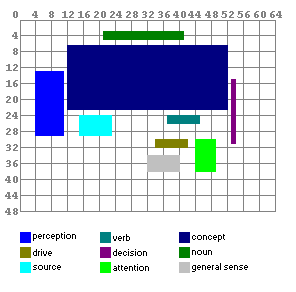
\includegraphics[width=0.95\textwidth]{img/brainmap.png}
\end{minipage} \hfill \begin{minipage}[ht]{0.575\textwidth}
	\small
	In this table, sizes are given in decimal, then in (hex). ~\\
	\begin{tabular}[h]{|c|c|c|c|c|c|c|c|c|}
		\hline
		Lobe ID	&	Gene \#	&	X		&	Y		&	Width	&	Height	&	Neurons	\\ \hline
		0		&	01		&	4 (04)	&	13 (0D)	&	7 (07)	&	16 (10)	&	112		\\ \hline
		1		&	02		&	34 (22)	&	30 (1E)	&	8 (08)	&	2 (02)	&	16		\\ \hline
		2		&	03		&	15 (0F)	&	24 (18)	&	8 (08)	&	5 (05)	&	40		\\ \hline
		3		&	04		&	37 (25)	&	24 (18)	&	8 (08)	&	2 (02)	&	16		\\ \hline
		4		&	08		&	21 (15)	&	3 (03)	&	20 (14)	&	2 (02)	&	40		\\ \hline
		5		&	09		&	32 (20)	&	34 (22)	&	8 (08)	&	4 (04)	&	32		\\ \hline
		6		&	05		&	53 (35)	&	15 (0F)	&	1 (01)	&	16 (10)	&	16		\\ \hline
		7		&	06		&	44 (2C)	&	30 (1E)	&	5 (05)	&	8 (08)	&	40		\\ \hline
		8		&	07		&	12 (0C)	&	6 (06)	&	40 (28)	&	16 (10)	&	640		\\ \hline
	\end{tabular}
\end{minipage} ~\\

\hrule ~\\

\begin{minipage}[ht]{0.40\textwidth}
	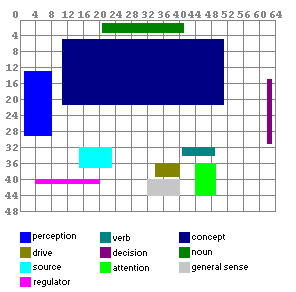
\includegraphics[width=0.95\textwidth]{img/brainmap2.png}
\end{minipage} \hfill \begin{minipage}[ht]{0.675\textwidth}
	\small
	In this table, sizes are given in decimal, then in (hex). ~\\
	\begin{tabular}[h]{|c|c|c|c|c|c|c|c|c|}
		\hline
		Lobe ID	&	Gene \#	&	X		&	Y		&	Width	&	Height	&	Neurons	\\ \hline
		0		&	01		&	1 (01)	&	13 (0D)	&	7 (07)	&	16 (10)	&	112		\\ \hline
		1		&	02		&	34 (22)	&	36 (24)	&	8 (08)	&	2 (02)	&	16		\\ \hline
		2		&	03		&	15 (0F)	&	32 (20)	&	8 (08)	&	5 (05)	&	40		\\ \hline
		3		&	04		&	37 (25)	&	32 (20)	&	8 (08)	&	2 (02)	&	16		\\ \hline
		4		&	08		&	21 (15)	&	1 (01)	&	20 (14)	&	2 (02)	&	40		\\ \hline
		5		&	09		&	32 (20)	&	40 (28)	&	8 (08)	&	4 (04)	&	32		\\ \hline
		6		&	05		&	62 (3E)	&	15 (0F)	&	1 (01)	&	16 (10)	&	16		\\ \hline
		7		&	06		&	44 (2C)	&	36 (24)	&	5 (05)	&	8 (08)	&	40		\\ \hline
		8		&	07		&	11 (0B)	&	5 (05)	&	40 (28)	&	16 (10)	&	640		\\ \hline
		9		&	0A		&	4 (04)	&	40 (28)	&	16 (10)	&	1 (01)	&	16		\\ \hline
	\end{tabular}
\end{minipage} ~\\

\clearpage

\subsubsection*{Lobes\markboth{Lobes}{Lobes}}
\addcontentsline{toc}{subsubsection}{Lobes}

\textbf{\large Gene Sequence}

Each lobe gene has six sections:
\begin{itemize}
	\item general -- count, positioning, regular header information (mutability, switch on, etc.).
	\item cell body -- cell body dynamics and cell state rule (SVRule).
	\item d0 growth -- class 0 dendrites growth, migration, and initial attachment details.
	\item d0 dynamics -- class 0 dendrites dynamics.
	\item d1 growth -- class 1 dendrites growth, migration, and initial attachment details.
	\item d1 dynamics -- class 1 dendrites dynamics. 
\end{itemize}

\begin{minipage}[ht]{0.40\textwidth}
	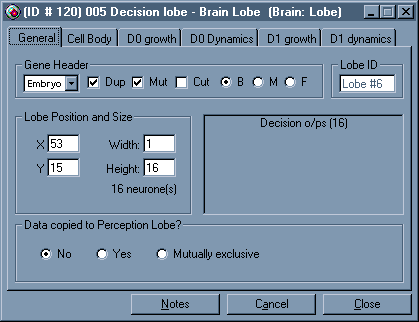
\includegraphics[width=0.95\textwidth]{img/gen00k1.png}
\end{minipage} \hfill \begin{minipage}[ht]{0.575\textwidth}
	\textbf{\large General} %% ~\\

	00 00 \#\# 00 00 sm xx yy ww hh pl ~\\

	00 -- gene type: brain ~\\
	00 -- gene subtype: lobe ~\\
	\#\# -- gene subtype number ~\\
	00 -- unknown / duplicate~\\
	00 -- switch on: embryo ~\\
	sm -- sex-dependence/mutability ~\\
	xx -- starting x position ~\\
	yy -- starting y position ~\\
	ww -- width ~\\
	hh -- height ~\\
	pl -- perception lobe link ~\\
\end{minipage} ~\\

\textsc{Gene Header}~\\

\textbf{sm -- sex dependence/mutability} --- No sex dependence. Lobes 1-4, 8, 9 -- no mutability. Lobe 7 -- mutable. Lobes 5 and 6 -- mutable, duplicable. See the Header page for a complete discussion of this byte. ~\\

\textsc{Lobe Position and Size}~\\
For a visual representation of lobe/neurone layout, see the \emph{Brainmap (C1 or C2)}. ~\\

\textbf{xx -- starting x position and yy -- starting y position} --- The Norn brain is laid out onto a 64x48 grid of neurons. These two characters locate the upper left corner of the block of neurons for each lobe, in the form of (xx,yy) on the grid. ~\\

\textbf{ww -- width and hh -- height} --- Each lobe consists of a block of neurons, and these two characters give the width and height of that block. The total number of neurons in a lobe is equal to the width times the height. ~\\

\textsc{Data copied to Perception Lobe?}~\\ 

\textbf{pl -- perception lobe link}
\begin{itemize}
	\item No (00)
	\item Yes (01)
	\item Mutually exclusive (02)
\end{itemize} ~\\

\clearpage

\begin{minipage}[ht]{0.40\textwidth}
	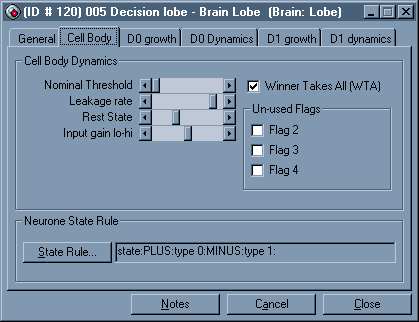
\includegraphics[width=0.95\textwidth]{img/gen00k2.png}
\end{minipage} \hfill \begin{minipage}[ht]{0.575\textwidth}
	\textbf{\large Cell Body} %% ~\\

	nt lk rs ig sr sr sr sr sr sr sr sr wt ~\\

	nt -- nominal threshold ~\\
	lk -- leakage rate ~\\
	rs -- rest state ~\\
	ig -- input gain lo-hi ~\\
	sr -- state rule ~\\
	wt -- winner takes all (WTA) ~\\
\end{minipage} ~\\

\textbf{\large Notes}

\textsc{Cell Body Dynamics} -- Specifies neurone properties. ~\\

\textbf{nt -- nominal threshold} --- A neurone will fire if its state rises above the threshold. Ranges from 00 to FF. ~\\

\textbf{lk -- leakage rate} --- Ranges from FF to 00. ~\\

\textbf{rs -- rest state} --- Ranges from 00 to FF. ~\\

\textbf{ig -- input gain lo-hi} ---	Ranges from 00 to FF. ~\\

\textbf{wt -- winner takes all (WTA)} --- WTA stands for "Winner Takes All." According to the Genetics Kit, when set (01), this means that all but the strongest-firing cell in the lobe is suppressed. This function can be used to decide which action or object wins the vote (in Decision and Attention lobes).
\begin{itemize}
	\item 00 -- no
	\item 01 -- yes
\end{itemize} ~\\

\textsc{Neurone State Rule} -- Used to calculate the new state of every neurone each "tick" (about 4 times a second in Creatures).

\textbf{sr -- state rule} --- State Variable Rules (SVRules) are used to control synaptic behavior and to compute a neurone's state about four times every second. They are made up of up to eight "interpreted opcodes and operands," with the <end> marker used to mark the end of the rule.

\begin{verbatim}
	For example:
		09	17   0C	 18	0D	00	00	00
		state:PLUS:type 0:MINUS:type1:<end>:<end>:<end>

	 Class 0 inputs are excitatory / Class 1 inputs are inhibitory.
	 [newstate = state + class0 -- class1]
\end{verbatim}

\clearpage

\begin{minipage}[ht]{0.40\textwidth}
	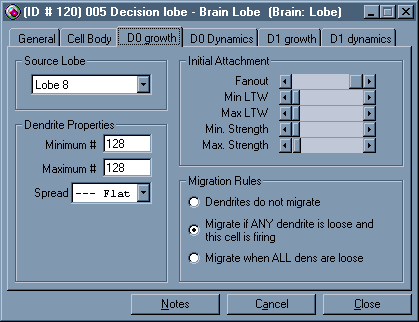
\includegraphics[width=0.95\textwidth]{img/gen00k3.png}
\end{minipage} \hfill \begin{minipage}[ht]{0.575\textwidth}
	\textbf{\large D0 Growth} %% ~\\

	sl ld ud sp fo ll ul ls us mr ~\\

	sl -- source lobe ~\\
	ld -- min \# dendrites ~\\
	ud -- max \# dendrites ~\\
	sp -- spread ~\\
	fo -- fanout ~\\
	ll -- min LTW ~\\
	ul -- max LTW ~\\
	ls -- min Strength ~\\
	us -- max Strength ~\\
	mr -- migration rule ~\\
\end{minipage} ~\\

\textbf{\large Notes} ~\\

\textsc{Source Lobe} -- The source lobe for the dendrite connections for these dendrites. ~\\

\textbf{sl -- source lobe} --- \emph{One of the lobe's number...} ~\\

\textsc{Dendrite Properties} -- The distribution of dendrites, and the minimum and maximum allowed. ~\\

\textbf{ld -- min \# dendrites} --- No idea what the upper limit of the range for this might be. ~\\

\textbf{ud -- max \# dendrites} --- No idea what the upper limit of the range for this might be. ~\\

\textbf{sp -- spread} --- \emph{Possible values are "Flat / Normal / Saw / waS". } ~\\

\textsc{Initial Attachment} -- Properties for how dendrites wire themselves to neurones. ~\\

\textbf{fo -- fanout} --- Appears to range from 00 to 08. ~\\

\textbf{ll -- min LTW} --- Ranges from 00 to FF. ~\\

\textbf{ul -- max LTW} --- Ranges from 00 to FF. ~\\

\textbf{ls -- min Strength} --- Ranges from 00 to FF. ~\\

\textbf{us -- max Strength} --- Ranges from 00 to FF. ~\\

\textsc{Migration Rules} -- The conditions under which dendrites migrate and find new connections. ~\\

\textbf{mr -- migration rule}
\begin{itemize}
	\item 00 -- Dendrites do not migrate
	\item 01 -- Migrate if ANY dendrite is loose and this cell is firing
	\item 02 -- Migrate when ALL dens are loose
\end{itemize}

\clearpage

\begin{minipage}[ht]{0.40\textwidth}
	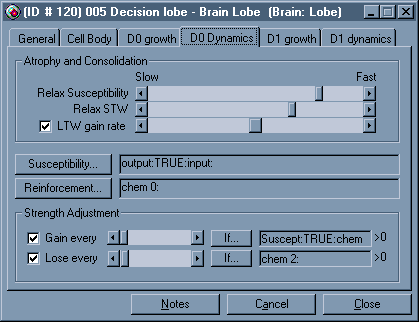
\includegraphics[width=0.95\textwidth]{img/gen00k4.png}
\end{minipage} \hfill \begin{minipage}[ht]{0.575\textwidth}
	\textbf{\large D0 Dynamics} %% ~\\

	a1 a2 a3 ~\\
	ge gr gr gr gr gr gr gr gr le lr lr lr lr lr lr lr lr ~\\
	ss ss ss ss ss ss ss ss rr rr rr rr rr rr rr rr ~\\

	a1 -- relax susceptibility ~\\
	a2 -- relax STW ~\\
	a3 -- LTW gain rate ~\\
	ge -- gain every... ~\\
	gr -- gain rule ~\\
	le -- lose every... ~\\
	lr -- lose rule ~\\
	ss -- susceptibility ~\\
	rr -- reinforcement ~\\
\end{minipage} ~\\

\textbf{\large Notes}~\\

\textsc{Atrophy and Consolidation} -- Information covering the atrophy and strengthening properties for dendrite connections. ~\\

\textbf{a1 -- relax susceptibility} --- Ranges from FF (slow) to 00 (fast). ~\\

\textbf{a2 -- relax STW} --- Ranges from FF (slow) to 00 (fast). ~\\

\textbf{a3 -- LTW gain rate} --- Ranges from FF (slow) to 00 (fast). ~\\

\textsc{Susceptibility/Reinforcement}~\\

\textbf{ss -- susceptibility} --- Another (optional) eight byte State Variable Rule (SVR) affecting the susceptibility of the dendrite link strength. %% ~\\
\begin{verbatim}
	For example:
		0A	 16   10	00	00	00	00	00
		output:TRUE:input:MINUS:<end>:<end>:<end>:<end>
\end{verbatim}

\textbf{rr -- reinforcement} --- Another (optional) eight byte State Variable Rule (SVR) affecting the reinforcement of the dendrite link strength. %% ~\\
\begin{verbatim}
	For example:
		05	 00	00	00	00	00	00	00
		chem 0:<end>:<end>:<end>:<end>:<end>:<end>:<end>
\end{verbatim}

\textsc{Strength Adjustment}~\\

\textbf{ge -- gain every...} --- Gain every \# if the value calculated by the gain rule is > 0. Range for \# is unknown. ~\\

\textbf{gr -- gain rule} --- Another eight byte State Variable Rule (SVR), used to control Strength gain. %% ~\\
\begin{verbatim}
	For example:
		12	16	05	16	13	00	00	00	
		Suscept:TRUE:chem 0:TRUE:STW:<end>:<end>:<end>
\end{verbatim}

\textbf{le -- lose every...} --- Lose every \# if the value calculated by the lose rule is > 0. Range for \# is unknown. ~\\

\textbf{lr -- lose rule} --- Another eight byte State Variable Rule (SVR), used to control Strength loss. %% ~\\
\begin{verbatim}
	For example:
		07	 00	00	00	00	00	00	00
		chem 2:<end>:<end>:<end>:<end>:<end>:<end>:<end>
\end{verbatim}


\begin{minipage}[ht]{0.45\textwidth}
	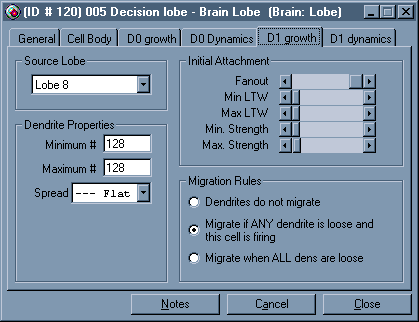
\includegraphics[width=0.95\textwidth]{img/gen00k5.png}~\\
	\textbf{\large D1 Growth} ~\\
	Repeat 10 bytes as noted in Dendrite 0 Growth above.
\end{minipage} \hfill \begin{minipage}[ht]{0.45\textwidth}
	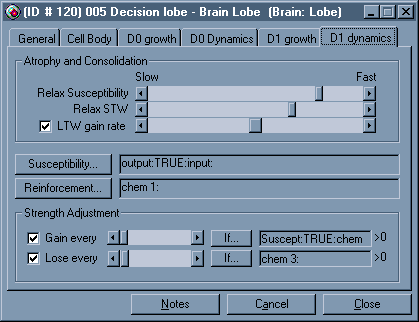
\includegraphics[width=0.95\textwidth]{img/gen00k6.png} ~\\
	\textbf{\large D1 Dynamics} ~\\
	Repeat 37 bytes as noted in Dendrite 0 Dynamics above.
\end{minipage} ~\\

%% \subsubsection*{Organ\markboth{Organ}{Organ}}
%% \addcontentsline{toc}{subsubsection}{Organ}

\clearpage

\subsection*{Biochemistry\markboth{Biochemistry}{Biochemistry}}
\addcontentsline{toc}{subsection}{Biochemistry}

\subsubsection*{Receptors\markboth{Receptors}{Receptors}}
\addcontentsline{toc}{subsubsection}{Receptors}

\begin{minipage}[ht]{0.40\textwidth}
	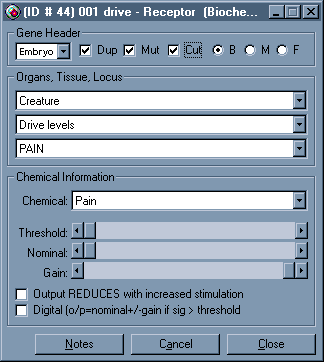
\includegraphics[width=0.95\textwidth]{img/gen10k.png}
\end{minipage} \hfill \begin{minipage}[ht]{0.575\textwidth}
	\textbf{\large Gene Sequence} %% ~\\
	
	01 00 \#\# 00 so sm \emph{mr} l1 l2 l3 cr tt no gg op ~\\

	01 -- gene type: biochemistry ~\\
	00 -- gene subtype: receptor ~\\
	\#\# -- gene subtype number ~\\
	00 -- unknown / duplicate ~\\
	so -- switch on: embryo ~\\
	sm -- sex-dependence/mutability ~\\
	\emph{mr -- mutation rate (C2 ONLY)} ~\\
	l\# -- locus of attachment ID ~\\
	cr -- chemical received ~\\
	tt -- threshold ~\\
	no -- nominal ~\\
	gg -- gain ~\\
	op -- output~\\
\end{minipage} ~\\

\textbf{\large Notes}

%% \textbf{sm -- sex dependence/mutability} --- See the Header page for a complete discussion of this byte.

\textbf{l\# -- locus ID} --- The locus of attachment of the chemo-receptor object. This three-character Locus ID represents 'organ,' 'tissue,' and 'site.'
\emph{See the LOA -- Receptors (C1 or C2) for the complete listing. }

\textbf{cr -- chemical received} --- The chemical that binds to the receptor and triggers its 'firing' -- i.e. the chemical monitored by the receptor.
\emph{See the ChemList (C1 or C2) for a listing of all the chemicals in Creatures.}

\textbf{tt -- threshold} --- The threshold is the level of chemical that must be present before the neuron bearing the bound receptor (the 'locus' above) will 'fire' (be activated).

According to the Creatures Developers Resource, the following formulas are used for calculating the new value of the locus when the amount of chemical exceeds the threshold:

%% \begin{math}
	Digital: $new value = nominal + (gain * R)$ ~\\
	Analog: $new value = nominal + (((amount -- threshold) * gain/255) * R)$ ~\\
	where R is either 1 or -1 (see op -- output below).
%% \end{math}

\textbf{no -- nominal} --- The 'nominal' of the receptor -- the amount to stimulate the locus if the chemical does not exceed the threshold. See the formulae above.

\textbf{gg -- gain} --- The 'gain' of the receptor -- the amount to stimulate the locus if the chemical does exceed the threshold. See the formulae above.

\textbf{op -- output} --- There are two check boxes on the Receptor gene editor:
\begin{itemize}
	\item[$\bullet$] Output REDUCES with increased stimulation
	\item[$\bullet$] Digital ($o/p = nominal +/- gain if sig > threshold$)
\end{itemize}

The first option determines whether the 'firing' of the neuron results in an increase in the value for the locus or in a decrease (listed as R in the formulae above).

The second option sets a receptor as Digital -- when unchecked, receptors are Analog. This choice determines which formula is used to calculate the new value for the receptor.

All the observed values in the byte can be explained with the last two bits:

\begin{minipage}[ht]{0.325\textwidth}
	\begin{tabular}[c]{ c c c c c c c c c c }
		bit & \# & 7 & 6 & 5 & 4 & 3 & 2 & 1 & 0 \\
		\hline
		00 & -- & 0 & 0 & 0 & 0 & 0 & 0 & 0 & 0 \\
		01 & -- & 0 & 0 & 0 & 0 & 0 & 0 & 0 & 1 \\
		02 & -- & 0 & 0 & 0 & 0 & 0 & 0 & 1 & 0 \\
		03 & -- & 0 & 0 & 0 & 0 & 0 & 0 & 1 & 1 \\
	\end{tabular}
\end{minipage} \hfill \begin{minipage}[ht]{0.175\textwidth}
	\footnotesize
	Bit 0 -- Reduces ~\\
	Bit 1 -- Digital ~\\
	\vfill
\end{minipage} \hfill \begin{minipage}[ht]{0.45\textwidth}
	\small
	In summary: ~\\
	\begin{tabular}[c]{ c c c c c c }
		01	&	=	&	Reduces		&				&				&			\\
		02	&	=	&				&	Digital		&				&			\\
		03	&	=	&	Reduces		&	Digital		&				&			\\
	\end{tabular}
\end{minipage} ~\\

\subsubsection*{Emitters\markboth{Emitters}{Emitters}}
\addcontentsline{toc}{subsubsection}{Emitters}

\begin{minipage}[ht]{0.40\textwidth}
	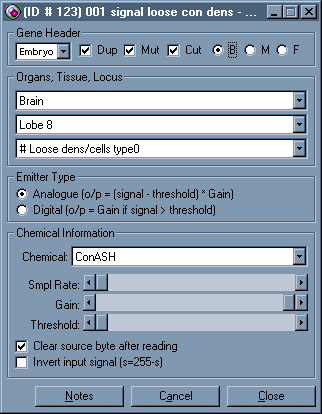
\includegraphics[width=0.95\textwidth]{img/gen11k.png}
\end{minipage} \hfill \begin{minipage}[ht]{0.575\textwidth}
	\textbf{\large Gene Sequence} %% ~\\
	
	01 01 \#\# 00 so sm \emph{mr} l1 l2 l3 ce tt sr gg et ~\\

	01 -- gene type: biochemistry ~\\
	01 -- gene subtype: emitter ~\\
	\#\# -- gene subtype number ~\\
	00 -- unknown / duplicate ~\\
	so -- switch on ~\\
	sm -- sex-dependence/mutability ~\\
	\emph{mr} -- mutation rate (C2 ONLY) ~\\
	l\# -- locus of attachment ID ~\\
	ce -- chemical emitted ~\\
	tt -- threshold ~\\
	sr -- smpl rate ~\\
	gg -- gain ~\\
	et -- emitter type ~\\
\end{minipage} ~\\

\textbf{\large Notes}

%% \textbf{sm -- sex dependence/mutability} --- See the Header page for a complete discussion of this byte.

\textbf{l\# -- locus ID} --- The locus of attachment of the chemo-emitter object. This three-character Locus ID represents 'organ,' 'tissue,' and 'site.' 
\emph{See the LOA -- Emitters (C1 or C2 ) for the complete listing.}

\textbf{ce -- chemical emitted} --- The chemical emitted when the chemical emitter binds to a cell in the brain. 
\emph{See the ChemList (C1 or C2) for a listing of all the chemicals in Creatures. }

\textbf{tt -- threshold} --- Ranges from 00 to FF. Whether the emitter is analog or digital determines how it is combined with the current signal level and the gain to calculate output -- see the 'emitter type' below.

\textbf{sr -- sample rate} --- Ranges from 00 to FF.

\textbf{gg -- gain} --- Ranges from 00 to FF. Whether the emitter is analog or digital determines how it is combined with the current signal level and the threshold to calculate output -- see the 'emitter type' below.

\textbf{et -- emitter type} --- There is a set of two radio buttons on the Emitter gene editor, indicating that the 'emitter type' will be either analog or digital.
\begin{itemize}
	\item Analog $(o/p = (signal -- threshold) * Gain)$
	\item Digital $(o/p = Gain if signal > threshold)$
\end{itemize}

In addition, there are two check boxes below the chemical information:
\begin{itemize}
	\item Clear source byte after reading
	\item Invert input signal ($s=255-s$)
\end{itemize}

All the observed values can be explained with the last three bits of the byte (with analog as the default emitter type):

\begin{minipage}[ht]{0.325\textwidth}
	\begin{tabular}[c]{ c c c c c c c c c c }
		bit & \# & 7 & 6 & 5 & 4 & 3 & 2 & 1 & 0 \\
		\hline
		00 & -- & 0 & 0 & 0 & 0 & 0 & 0 & 0 & 0 \\
		01 & -- & 0 & 0 & 0 & 0 & 0 & 0 & 0 & 1 \\
		02 & -- & 0 & 0 & 0 & 0 & 0 & 0 & 1 & 0 \\
		03 & -- & 0 & 0 & 0 & 0 & 0 & 0 & 1 & 1 \\
		04 & -- & 0 & 0 & 0 & 0 & 0 & 1 & 0 & 0 \\
		06 & -- & 0 & 0 & 0 & 0 & 0 & 1 & 1 & 0 \\
	\end{tabular}
\end{minipage} \hfill \begin{minipage}[ht]{0.175\textwidth}
	\footnotesize
	Bit 0 -- Clear ~\\
	Bit 1 -- Digital ~\\
	Bit 2 -- Invert ~\\
	\vfill
\end{minipage} \hfill \begin{minipage}[ht]{0.45\textwidth}
	\small
	In summary: ~\\
	\begin{tabular}[c]{ c c c c c c }
		00	&	=	&	Analog		&				&				&			\\
		01	&	=	&	Analog		&	Clear		&				&			\\
		02	&	=	&	Digital		&				&				&			\\
		03	&	=	&	Digital		&	Clear		&				&			\\
		04	&	=	&	Analog		&	Invert		&				&			\\
		06	&	=	&	Digital		&	Invert		&				&			\\
	\end{tabular}
\end{minipage} ~\\

\subsubsection*{Reactions\markboth{Reactions}{Reactions}}
\addcontentsline{toc}{subsubsection}{Reactions}

\begin{minipage}[ht]{0.40\textwidth}
	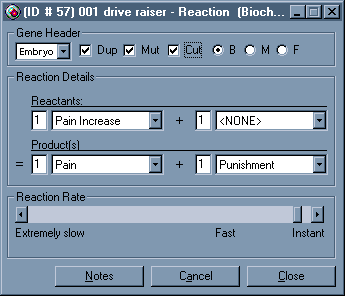
\includegraphics[width=0.95\textwidth]{img/gen12k.png}
\end{minipage} \hfill \begin{minipage}[ht]{0.575\textwidth}
	\textbf{\large Gene Sequence} %% ~\\

	01 02 \#\# 00 so sm \emph{mr} pa ca pb cb pc cc pd cd rr ~\\

	01 -- gene type: biochemistry ~\\
	02 -- gene subtype: reaction ~\\
	\#\# -- gene subtype number ~\\
	00 -- unknown / duplicate ~\\
	so -- switch on ~\\
	sm -- sex-dependence/mutability ~\\
	\emph{mr -- mutation rate (C2 ONLY)} ~\\
	p$ -- proportion of chemical (A-D) ~\\
	c$ -- chemical (A-D) ~\\
	rr -- reaction rate  ~\\
\end{minipage} ~\\

\textbf{\large Notes}

%% \textbf{sm -- sex dependence/mutability} --- See the Header page for a complete discussion of this byte.

\textbf{p\$ -- proportion of chemical (A-D)} --- The proportion of a chemical in the reaction (where \$ stands for either A, B, C, or D).

\textbf{c\$ -- chemical (A-D)} --- Each chemical in the reaction (where \$ stands for either A, B, C, or D). 
\emph{See the ChemList (C1 or C2) for a listing of all the chemicals in Creatures. }

\textbf{rr -- reaction rate} --- The rate of the reaction, which is concentration dependent and thus exponential over time.

\textbf{\large Example(s)}

\emph{See the Formulae (C1 or C2) page for a listing of the reactions in scientific notation. }
 
\emph{See also the Mutations (C1) page, as many of the 'named' mutations are changes in Reaction genes. }

\subsubsection*{Half-Lives\markboth{Half-Lives}{Half-Lives}}
\addcontentsline{toc}{subsubsection}{Half-Lives}

\begin{minipage}[ht]{0.40\textwidth}
	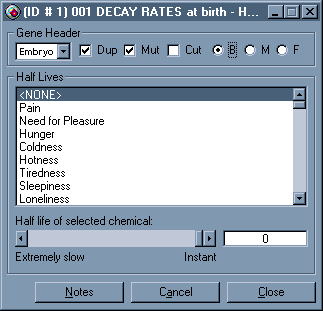
\includegraphics[width=0.95\textwidth]{img/gen13k.png}
\end{minipage} \hfill \begin{minipage}[ht]{0.575\textwidth}
	\textbf{\large Gene Sequence} %% ~\\

	01 03 01 00 00 sm \emph{80} \textbf{[255 more characters]} ~\\

	01 -- gene type: biochemistry ~\\
	03 -- gene subtype: half-lives ~\\
	01 -- gene subtype number ~\\
	00 -- unknown / duplicate ~\\
	00 -- switch on: embryo ~\\
	sm -- sex-dependence/mutability ~\\
	\emph{80 -- mutation rate (C2 ONLY)} ~\\
	\textbf{[ -- ]} -- half-life for each chemical ~\\
\end{minipage} ~\\

\textbf{\large Notes}

%% \textbf{sm -- sex dependence/mutability} --- No sex dependence. See the Header page for a complete discussion of this byte.

\textbf{[ ] -- half-life for each chemical} --- There are 255 (256 in C1) additional characters after the 'header,' corresponding to the 255 chemicals in the ChemList (C1 or C2). Half-life (how quickly the chemical degrades) ranges from 00 (instant) to FF (extremely slow).

\subsubsection*{Initial Concentrations\markboth{Initial Concentrations}{Initial Concentrations}}
\addcontentsline{toc}{subsubsection}{Initial Concentrations}

\begin{minipage}[ht]{0.40\textwidth}
	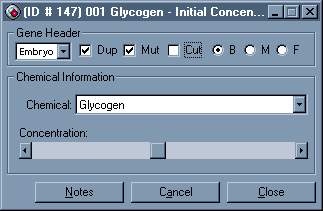
\includegraphics[width=0.95\textwidth]{img/gen14k.png}
\end{minipage} \hfill \begin{minipage}[ht]{0.575\textwidth}
	\textbf{\large Gene Sequence} %% ~\\

	01 04 \#\# 00 00 sm \emph{mr} cc ic ~\\

	01 -- gene type: biochemistry ~\\
	04 -- gene subtype: initial concentration ~\\
	\#\# -- gene subtype number ~\\
	00 -- unknown / duplicate ~\\
	00 -- switch on: embryo ~\\
	sm -- sex-dependence/mutability ~\\
	\emph{mr -- mutation rate (C2 ONLY)} ~\\
	cc -- chemical ~\\
	ic -- initial concentration ~\\ 
\end{minipage} ~\\

\textbf{\large Notes}

%% \textbf{sm -- sex dependence/mutability} --- See the Header page for a complete discussion of this byte.

\textbf{cc -- chemical} --- \emph{See the ChemList (C1 or C2) for a listing of all the chemicals in Creatures.} ~\\ 

\textbf{ic -- initial concentration} --- The amount of the chemical present in the Norn at birth, ranging between 00 and FF. ~\\ 

\textbf{\large Example(s)} ~\\ 
	01 04 01 00 00 03 3B 7A --- This C1 gene sequence sets the initial concentration of glycogen (chemical 3B). ~\\ 
	01 04 05 00 00 07 F0 82 --- This C1 gene sequence sets the initial concentration of Antibody 0 (chemical F0). ~\\  

\clearpage

\subsection*{Creature\markboth{Creature}{Creature}}
\addcontentsline{toc}{subsection}{Creature}

\subsubsection*{Stimuli\markboth{Stimuli}{Stimuli}}
\addcontentsline{toc}{subsubsection}{Stimuli}

\begin{minipage}[ht]{0.40\textwidth}
	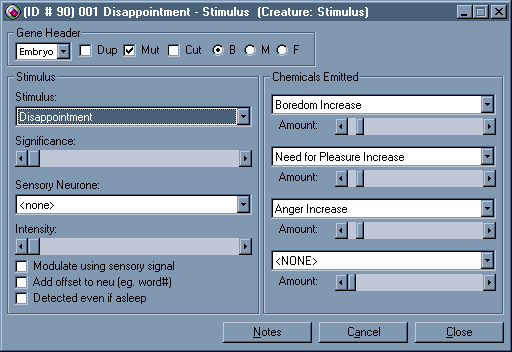
\includegraphics[width=0.95\textwidth]{img/gen20k.png}
\end{minipage} \hfill \begin{minipage}[ht]{0.575\textwidth}
	\textbf{\large Gene Sequence} %% ~\\

	02 00 \#\# 00 so sm \emph{mr} st sg sn ii ff c0 a0 c1 a1 c2 a2 c3 a3 ~\\

	02 -- gene type: creature ~\\
	00 -- gene subtype: appearance ~\\
	\#\# -- gene subtype number ~\\
	00 -- unknown / duplicate ~\\
	so -- switch on ~\\
	sm -- sex-dependence/mutability ~\\
	\emph{mr -- mutation rate (C2 ONLY)} ~\\
	st -- stimulus ~\\
	sg -- significance ~\\
	sn -- sensory neurone ~\\
	ii -- intensity ~\\
	ff -- features ~\\
	c\# -- chemical emitted ~\\
	a\# -- amount of chemical emitted  ~\\
\end{minipage} ~\\

\subsubsection*{Genus\markboth{Genus}{Genus}}
\addcontentsline{toc}{subsubsection}{Genus}

\begin{minipage}[ht]{0.40\textwidth}
	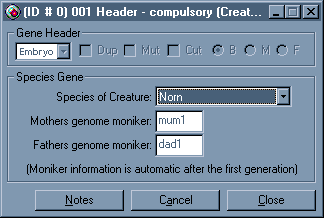
\includegraphics[width=0.95\textwidth]{img/gen21k.png}
\end{minipage} \hfill \begin{minipage}[ht]{0.575\textwidth}
	\textbf{\large Gene Sequence} %% ~\\

	02 01 \#\# 00 00 00 \emph{80} gg mm mm mm mm dd dd dd dd ~\\

	02 -- gene type: creature ~\\
	01 -- gene subtype: genus ~\\
	\#\# -- gene subtype number ~\\
	00 -- unknown / duplicate ~\\
	00 -- switch on: embryo ~\\
	00 -- sex-dependence/mutability: none ~\\
	\emph{80 -- mutation rate (C2 ONLY)} ~\\
	gg -- genus ~\\
	mm -- mum moniker ~\\
	dd -- dad moniker ~\\  
\end{minipage} ~\\

\textbf{\large Notes}~\\

gg - genus

    00 - Norn
    01 - Grendel
    02 - Ettin (C2 ONLY) 

mm - mum moniker

These four characters are a literal hexadecimal translation of the four character moniker that uniquely identifies each Creature on your hard drive (see the Science Kit). Generation 1 Norns are created by combining the mum#.gen and dad#.gen files (where # = 1 to 6).

dd - dad moniker

Ditto for Dad. Grendels don't have dads, poor things.
Example(s)

02 01 01 00 00 00 00 6D 75 6D 31 64 61 64 31
This is a C1 Norn with parents mum1 and dad1.

02 01 01 00 00 00 00 39 4F 49 48 36 53 56 50
This is a C1 Norn with parents 9OIH and 6SVP. 

\subsubsection*{Appearances\markboth{Appearances}{Appearances}}
\addcontentsline{toc}{subsubsection}{Appearances}

\begin{minipage}[ht]{0.40\textwidth}
	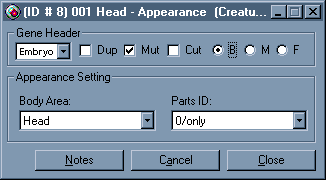
\includegraphics[width=0.95\textwidth]{img/gen22k.png}
\end{minipage} \hfill \begin{minipage}[ht]{0.575\textwidth}
	\textbf{\large Gene Sequence} %% ~\\

	02 02 \#\# 00 00 sm 80 bb st \emph{00} ~\\

	02 -- gene type: creature ~\\
	02 -- gene subtype: appearance ~\\
	\#\# -- gene subtype number ~\\
	00 -- unknown / duplicate ~\\
	00 -- switch on: embryo ~\\
	sm -- sex-dependence/mutability ~\\
	\emph{80 -- mutation rate (C2 only)} ~\\
	bb -- body location ~\\
	st -- sprite type ~\\
	\emph{00 -- unknown / duplicate (C2 only)} ~\\ 
\end{minipage} ~\\

\subsubsection*{Poses\markboth{Poses}{Poses}}
\addcontentsline{toc}{subsubsection}{Poses}

\begin{minipage}[ht]{0.40\textwidth}
	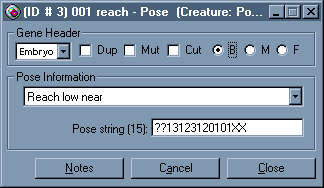
\includegraphics[width=0.95\textwidth]{img/gen23k.png}
\end{minipage} \hfill \begin{minipage}[ht]{0.575\textwidth}
	\textbf{\large Gene Sequence} %% ~\\
	
	02 03 \#\# 00 so 00 \emph{mr} pn ps ps ps ps ps ps ps ps ps ps ps ps ps ps ps ~\\
	
	02 -- gene type: creature ~\\
	03 -- gene subtype: pose ~\\
	\#\# -- gene subtype number ~\\
	00 -- unknown / duplicate ~\\
	so -- switch on ~\\
	00 -- sex-dependence/mutability: none ~\\
	\emph{mr -- mutation rate (C2 ONLY)} ~\\
	pn -- pose number ~\\
	ps -- pose string ~\\
\end{minipage} ~\\

\subsubsection*{Gaits\markboth{Gaits}{Gaits}}
\addcontentsline{toc}{subsubsection}{Gaits}

\begin{minipage}[ht]{0.40\textwidth}
	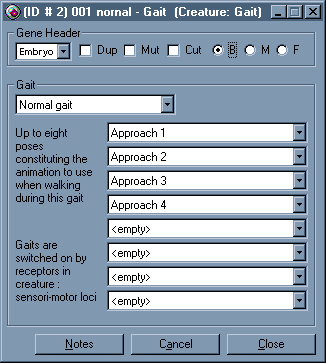
\includegraphics[width=0.95\textwidth]{img/gen24k.png}
\end{minipage} \hfill \begin{minipage}[ht]{0.575\textwidth}
	\textbf{\large Gene Sequence} %% ~\\

	02 04 \#\# 00 00 00 \emph{80} gn g1 g2 g3 g4 g5 g6 g7 g8 ~\\

	02 -- gene type: creature ~\\
	04 -- gene subtype: gait ~\\
	\#\# -- gene subtype number ~\\
	00 -- unknown / duplicate ~\\
	00 -- switch on: embryo ~\\
	00 -- sex-dependence/mutability: none ~\\
	\emph{80 -- mutation rate (C2 ONLY)} ~\\
	gn -- gait number ~\\
	g\# -- gait sequence ~\\  
\end{minipage} ~\\

\subsubsection*{Instincts\markboth{Instincts}{Instincts}}
\addcontentsline{toc}{subsubsection}{Instincts}

\begin{minipage}[ht]{0.40\textwidth}
	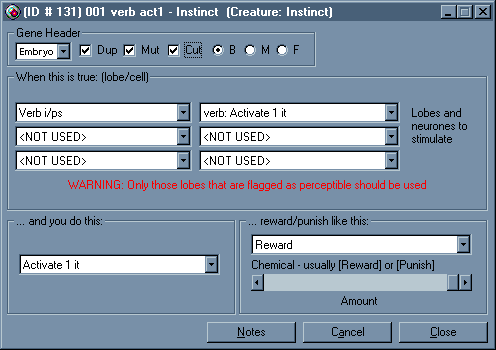
\includegraphics[width=0.95\textwidth]{img/gen25k.png}
\end{minipage} \hfill \begin{minipage}[ht]{0.575\textwidth}
	\textbf{\large Gene Sequence} %% ~\\

	02 05 \#\# 00 so sm \emph{mr} l1 c1 l2 c2 l3 c3 ca rp aa ~\\

	02 -- gene type: creature ~\\
	05 -- gene subtype: instinct ~\\
	\#\# -- gene subtype number ~\\
	00 -- unknown / duplicate ~\\
	so -- switch on ~\\
	sm -- sex-dependence/mutability ~\\
	\emph{mr -- mutation rate (C2 ONLY)} ~\\
	l\# -- lobe ~\\
	c\# -- cell ~\\
	ca -- creature action ~\\
	rp -- reward or punish ~\\
	aa -- amount ~\\

\end{minipage} ~\\

\clearpage

\subsubsection*{Pigment\markboth{Pigment}{Pigment}}
\addcontentsline{toc}{subsubsection}{Pigment}

\begin{minipage}[ht]{0.40\textwidth}
	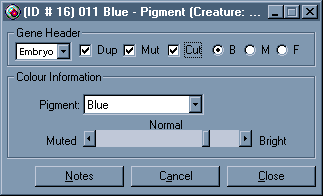
\includegraphics[width=0.95\textwidth]{img/gen26k.png}
\end{minipage} \hfill \begin{minipage}[ht]{0.575\textwidth}
	\textbf{\large Gene Sequence} %% ~\\

	02 06 \#\# 00 00 sm \emph{80} pp ii ~\\

	02 -- gene type: creature ~\\
	06 -- gene subtype: pigment ~\\
	\#\# -- gene subtype number ~\\
	00 -- unknown / duplicate ~\\
	00 -- switch on: embryo ~\\
	sm -- sex-dependence/mutability ~\\
	\emph{80 -- mutation rate (C2 ONLY)} ~\\
	pp -- pigment ~\\
	ii -- intensity  ~\\
\end{minipage} ~\\

\textbf{\large Notes} ~\\

\textbf{sm -- sex dependence/mutability} --- No sex dependence, and all three types of mutability (mutable, duplicable, deletable). See the Header page for a complete discussion of this byte. ~\\

\textbf{pp -- pigment}
\begin{itemize}
	\item 00 -- red
	\item 01 -- green
	\item 02 -- blue
\end{itemize}~\\

\textbf{ii -- intensity} --- As Sandra J. Linkletter deduced, this must represent the intensity of the color, using RGB light (thus 00 = black and FF = white). Apparently these values are added to a base raw umber color. ~\\

\textbf{general observations} --- Despite the names of the first three genes, currently all colors are present at birth, according to information Cyberlife gave Sandra. ~\\

\textbf{\large Example(s)}~\\
	02 06 05 00 00 07 00 11 --- This gene sets one of the C1 red pigments to intensity 11 (decimal 17). ~\\ 	
	02 06 0D 00 00 07 80 02 FF --- This gene sets one of the C2 blue pigments to intensity FF (decimal 255). ~\\  

\subsubsection*{Pigment Bleed\markboth{Pigment Bleed}{Pigment Bleed}}
\addcontentsline{toc}{subsubsection}{Pigment Bleed}

\begin{minipage}[ht]{0.40\textwidth}
	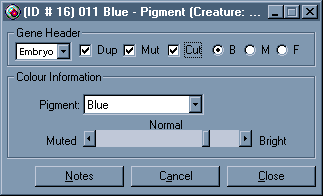
\includegraphics[width=0.95\textwidth]{img/gen26k.png}
\end{minipage} \hfill \begin{minipage}[ht]{0.575\textwidth}
	\textbf{\large Gene Sequence} %% ~\\

	02 07 \#\# 00 00 sm 80 rt sw ~\\

	02 -- gene type: creature ~\\
	07 -- gene subtype: pigment bleed ~\\
	\#\# -- gene subtype number ~\\
	00 -- unknown / duplicate ~\\
	00 -- switch on: embryo ~\\
	sm -- sex-dependence/mutability ~\\
	80 -- mutation rate ~\\
	rt -- rotation ~\\
	sw -- swap ~\\
\end{minipage} ~\\

\clearpage

\subsection*{Body:Organ\markboth{Body:Organ}{Body:Organ}}
\addcontentsline{toc}{subsection}{Body:Organ}



\clearpage

\section*{Section\markboth{Section}{Section}}
\addcontentsline{toc}{section}{Section}

\clearpage

%% \section*{Bibliography\markboth{Bibliography}{Bibliography}}
%% \addcontentsline{toc}{section}{Bibliography}
%% \bibliography{bibliography} %% .bib
%% \bibliographystyle{frplain} % plain or frplain

\end{document}
